\section{Odpowiedzi}

\subsection*{Gniazda klienckie TCP}
\begin{enumerate}[label=\textbf{3.\arabic*}]\setlength{\itemsep}{1em}
    \item    Aby przetestować poprawność swojego rozwiązania, możesz przeskanować swój własny komputer, żeby sprawdzić, czy skanowanie da taki sam wynik, jak Twój program. Do tego celu możesz wykorzystać np. narzędzie \texttt{nmap}. Zainstaluj \texttt{nmap}: \texttt{sudo apt install nmap}, a następnie wydaj polecenie: \texttt{nmap -p 22 localhost} (lub \texttt{nmap -p 22 127.0.0.1}) aby sprawdzić, czy port 22 jest otwarty na Twoim komputerze. Porównaj wynik z działaniem Twojego programu dla tego samego portu.  

\begin{figure}[h]
\caption{Wynik działania programu \texttt{nmap} dla lokalnej maszyny i portu \texttt{22}}
\centering
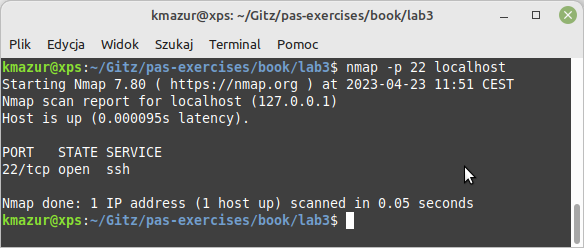
\includegraphics[scale=0.6]{./images/answers/ex3.1.png}
\end{figure}   
% #####################################################################################################

\item Możesz przetestować program używając swojego lokalnego adresu IPv6: \texttt{::1} lub \texttt{localhost} lub \\ \texttt{0000:0000:0000:0000:0000:0000:0000:0001}. 

\begin{figure}[h]
\caption{Wynik działania programu \texttt{nmap} dla lokalnej maszyny i portu \texttt{22}}
\centering
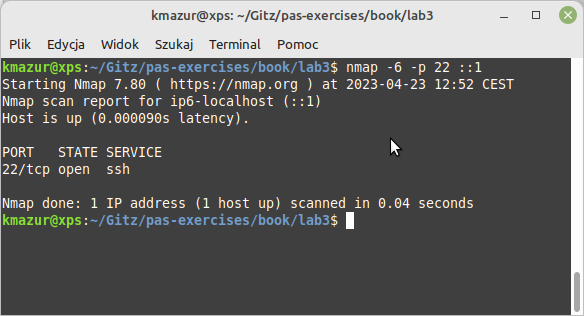
\includegraphics[scale=0.6]{./images/answers/ex3.2-nmap.png}
\end{figure}   
% #####################################################################################################

\newpage
\item Aby przetestować poprawność swojego rozwiązania, możesz przeskanować swój własny komputer, żeby sprawdzić, czy skanowanie da taki sam wynik, jak Twój program. Do tego celu możesz wykorzystać np. narzędzie \texttt{nmap}. Zainstaluj \texttt{nmap}: \texttt{sudo apt install nmap}, a następnie wydaj polecenie: \texttt{nmap -p1-65535 localhost} (lub \texttt{nmap -p1-65535 127.0.0.1}) aby sprawdzić, jakie porty są otwarte na Twoim komputerze. Porównaj wynik z działaniem Twojego programu dla tego samego portu.  

\begin{figure}[h]
\caption{Wynik działania programu \texttt{nmap} dla lokalnej maszyny i wszystkich jej portów}
\centering
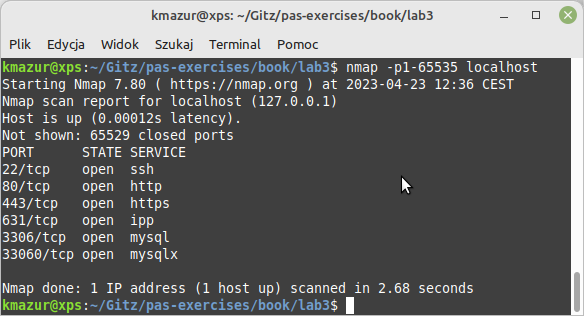
\includegraphics[scale=0.6]{./images/answers/ex3.3-nmap.png}
\end{figure}   
% #####################################################################################################

\item Aby przetestować poprawność swojego rozwiązania, możesz przeskanować swój własny komputer, żeby sprawdzić, czy skanowanie da taki sam wynik, jak Twój program. Do tego celu możesz wykorzystać np. narzędzie \texttt{nmap}. Zainstaluj \texttt{nmap}: \texttt{sudo apt install nmap}, a następnie wydaj polecenie: \texttt{nmap -6 -p1-65535 localhost} (lub \texttt{nmap -6 -p1-65535 ::1}) aby sprawdzić, jakie porty są otwarte na Twoim komputerze. Porównaj wynik z działaniem Twojego programu dla tego samego portu.  

\begin{figure}[h]
\caption{Wynik działania programu \texttt{nmap} dla lokalnej maszyny i wszystkich jej portów}
\centering
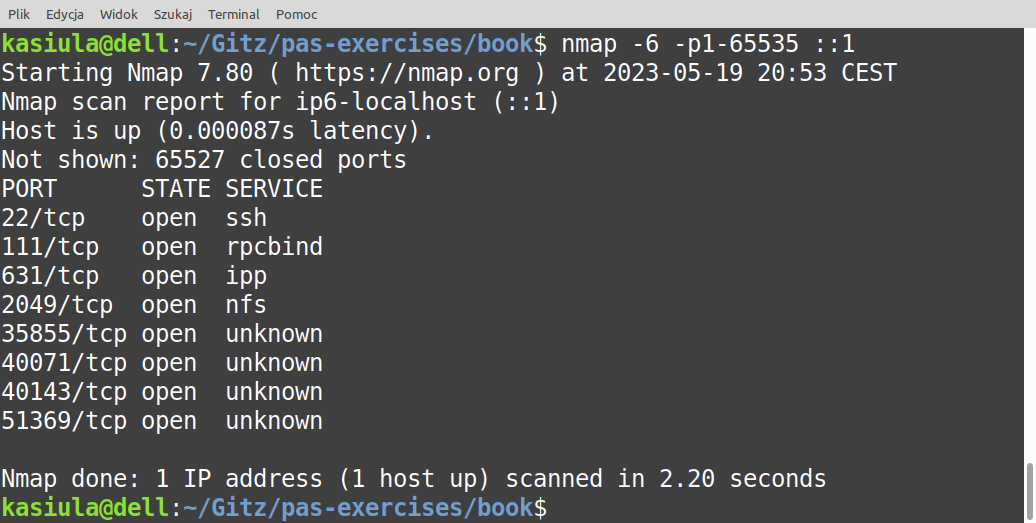
\includegraphics[scale=0.35]{./images/answers/ex3.4-nmap.png}
\end{figure}   
% #####################################################################################################

\item Aby przetestować poprawność swojego rozwiązania, możesz skorzystać z gotowego serwera, do którego może połączyć się Twój klient, aby pobrać aktualną datę i czas. Aby uruchomić serwer, zainstaluj \href{https://www.docker.com/}{Dockera}, a następnie w konsoli wydaj polecenia:

\begin{itemize}
\item Pobierz obraz serwera:\\ \texttt{docker pull mazurkatarzyna/pas-book-p1-ch3-ex5-server:latest}

\item Uruchom serwer za pomocą Dockera:\\ \texttt{docker run -dp 3005:3005 mazurkatarzyna/pas-book-p1-ch3-ex5-server}
\end{itemize}

\noindent Tak uruchomiony serwer działa na Twoim komputerze, jego adres IPv4 to \texttt{127.0.0.1} (\texttt{localhost}), numer portu to 3005.
% #####################################################################################################

\item Aby przetestować poprawność swojego rozwiązania, możesz skorzystać z gotowego serwera, do którego może połączyć się Twój klient, aby pobrać aktualną datę i czas. Aby uruchomić serwer, zainstaluj \href{https://www.docker.com/}{Dockera}, a następnie w konsoli wydaj polecenia:

\begin{itemize}
\item Pobierz obraz serwera:\\ \texttt{docker pull mazurkatarzyna/pas-book-p1-ch3-ex6-server:latest}

\item Uruchom serwer za pomocą Dockera:\\ \texttt{docker run -dp 3006:3006 mazurkatarzyna/pas-book-p1-ch3-ex6-server}
\end{itemize}

\noindent Tak uruchomiony serwer działa na Twoim komputerze, jego adres IPv6 to \texttt{::1} (\texttt{localhost}), numer portu to 3006.
% #####################################################################################################
\item Aby przetestować poprawność swojego rozwiązania, możesz skorzystać z gotowego serwera, do którego może połączyć się Twój klient, aby wysłać wiadomość. Aby uruchomić serwer, zainstaluj \href{https://www.docker.com/}{Dockera}, a następnie w konsoli wydaj polecenia:

\begin{itemize}
\item Pobierz obraz serwera:\\ \texttt{docker pull mazurkatarzyna/pas-book-p1-ch3-ex7-server:latest}

\item Uruchom serwer za pomocą Dockera:\\ \texttt{docker run -dp 3007:3007 mazurkatarzyna/pas-book-p1-ch3-ex7-server}
\end{itemize}

\noindent Tak uruchomiony serwer działa na Twoim komputerze, jego adres IPv4 to \texttt{127.0.0.1} (\texttt{localhost}), numer portu to 3007.
%#####################################################################################################

\item Aby przetestować poprawność swojego rozwiązania, możesz skorzystać z gotowego serwera, do którego może połączyć się Twój klient, aby wysłać wiadomość. Aby uruchomić serwer, zainstaluj \href{https://www.docker.com/}{Dockera}, a następnie w konsoli wydaj polecenia:

\begin{itemize}
\item Pobierz obraz serwera:\\ \texttt{docker pull mazurkatarzyna/pas-book-p1-ch3-ex8-server:latest}

\item Uruchom serwer za pomocą Dockera:\\ \texttt{docker run -dp 3008:3008 mazurkatarzyna/pas-book-p1-ch3-ex8-server}
\end{itemize}

\noindent Tak uruchomiony serwer działa na Twoim komputerze, jego adres IPv6 to \texttt{::1} (\texttt{localhost}), numer portu to 3008.
%#####################################################################################################
\item Aby przetestować poprawność swojego rozwiązania, możesz skorzystać z gotowego serwera, do którego może połączyć się Twój klient, aby wysłać wiadomość. Aby uruchomić serwer, zainstaluj \href{https://www.docker.com/}{Dockera}, a następnie w konsoli wydaj polecenia:

\begin{itemize}
\item Pobierz obraz serwera:\\ \texttt{docker pull mazurkatarzyna/pas-book-p1-ch3-ex9-server:latest}

\item Uruchom serwer za pomocą Dockera:\\ \texttt{docker run -dp 3009:3009 mazurkatarzyna/pas-book-p1-ch3-ex9-server}
\end{itemize}

\noindent Tak uruchomiony serwer działa na Twoim komputerze, jego adres IPv4 to \texttt{127.0.0.1} (\texttt{localhost}), numer portu to 3009.
%#####################################################################################################
\item Aby przetestować poprawność swojego rozwiązania, możesz skorzystać z gotowego serwera, do którego może połączyć się Twój klient, aby wysłać wiadomość. Aby uruchomić serwer, zainstaluj \href{https://www.docker.com/}{Dockera}, a następnie w konsoli wydaj polecenia:

\begin{itemize}
\item Pobierz obraz serwera:\\ \texttt{docker pull mazurkatarzyna/pas-book-p1-ch3-ex10-server:latest}

\item Uruchom serwer za pomocą Dockera:\\ \texttt{docker run -dp 3010:3010 mazurkatarzyna/pas-book-p1-ch3-ex10-server}
\end{itemize}

\noindent Tak uruchomiony serwer działa na Twoim komputerze, jego adres IPv6 to \texttt{::1} (\texttt{localhost}), numer portu to 3010.
%#####################################################################################################
\end{enumerate}
